\scanpage{70}
\mspage{34}
$4^\circ)$ \uline{Cas de} $\widehat M^!_{1,2}\simeq\widehat M^{\deleted{\unsure{!}}}_{1,I}$ $(\operatorname{card}I=2\deleted{\unsure{\}}},\ I=\{a,b\})$
\[
(83)\quad\left\{\diagram{\begin{tikzcd}[ampersand replacement=\&, column sep=18pt,row sep=14pt,
execute at end picture={
\draw ([xshift=9pt]scan070-codim-zero.east |- scan070-codim-zero.north) -- ([xshift=9pt]scan070-codim-zero.east |- current bounding box.south);
\draw ([xshift=-9pt]scan070-p-one.west |- scan070-codim-zero.north) -- ([xshift=-9pt,yshift=-4pt]scan070-p-one.west |- current bounding box.south);
}]
|[alias=scan070-codim-zero]|\text{codim }0\&\text{codim }1\&\text{codim }2\\
\& G_0={\figure{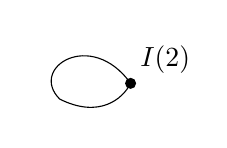
\begin{tikzpicture}[baseline=-2pt]\draw (0,0)..controls(-.5,.7)and(-1.3,.2)..(-.9,-.2)..controls(-.4,-.45)and(-.1,-.2)..(0,0);\fill(0,0) circle(2pt);\node[above right]at(0,0){$I(2)$};\end{tikzpicture}}}\arrow[r,"2"]\arrow[dr,"1"']\&
{\figure{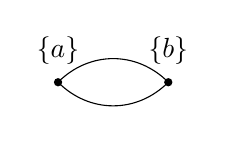
\begin{tikzpicture}[baseline=-2pt]\draw (0,0)..controls(.4,.4)and(1,.4)..(1.4,0);\draw (0,0)..controls(.4,-.4)and(1,-.4)..(1.4,0);\fill(0,0)circle(1.5pt);\fill(1.4,0)circle(1.5pt);\node[above]at(0,.1){$\{a\}$};\node[above]at(1.4,.1){$\{b\}$};\end{tikzpicture}}}=P_0\\
{\figure{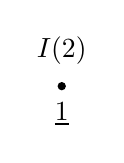
\begin{tikzpicture}[baseline=-2pt]\fill(0,0)circle(1.5pt);\node[above]at(0,.15){$I(2)$};\node[below]at(0,-.08){$\underline1$};\end{tikzpicture}}}\&
G_1={\figure{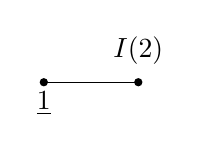
\begin{tikzpicture}[baseline=-2pt]\draw(0,0)--(1.2,0);\fill(0,0)circle(1.5pt);\fill(1.2,0)circle(1.5pt);\node[below]at(0,0){$\underline1$};\node[above]at(1.2,.1){$I(2)$};\end{tikzpicture}}}\arrow[r,"1"]\&
|[alias=scan070-p-one]|{\figure{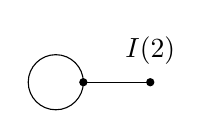
\begin{tikzpicture}[baseline=-2pt]\draw (0,0) circle(.35);\draw (.35,0)--(1.2,0);\fill(.35,0)circle(1.5pt);\fill(1.2,0)circle(1.5pt);\node[above]at(1.2,.1){$I(2)$};\end{tikzpicture}}}=P_1
\end{tikzcd}}\right.
\]
\margin{$D_\circ$ ``D boucle''\quad $D_{\bullet-\bullet}$ ``D segment''}
Il y a deux diviseurs à l'infini, \inserted{$D_\circ$ et $D_{\bullet-\bullet}$,} et deux points \inserted{critiques} à l'infini, \deleted{dont}\inserted{$P_0$ et $P_1$,} l'un \inserted{$P_0$} est contenu dans $D_\circ$ et dans $D_{\bullet-\bullet}$, et l'autre n'est contenu que dans $D_{\bullet-\bullet}$.

Essayons de \inserted{bien} saisir la structure de la multiplicité schématique à l'infini $\widehat M^\infty_{1,I}\simeq\widehat M^{!\,\infty}_{1,2}$, qui est la réunion amalgamée des deux multiplicités lisses \deleted{\unsure{$\widehat M$}} $D_\circ$ et $D_{\bullet-\bullet}$.
$D_\circ$ est isomorphe à $(\widehat M^{\unsure{!}}_{G_0},\Gamma^!_0)$, où $G_0$ est le \inserted{MD-}graphe
\figure{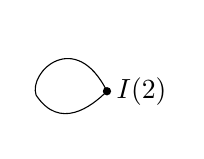
\begin{tikzpicture}[baseline=-2pt]\draw (0,0)..controls(-.4,.8)and(-1,.25)..(-.9,-.05)..controls(-.6,-.5)and(-.2,-.2)..(0,0);\fill(0,0)circle(1.5pt);\node[right]at(0,0){$I(2)$};\end{tikzpicture}},
$\Gamma_0$ son groupe d'automorphismes, et $\Gamma^!_0=\operatorname{Ker}(\Gamma_0\longrightarrow\mathfrak S_{I(G_0)})\simeq\mathbf Z/2$.
D'ailleurs $\widehat M_{G_0}\simeq\widehat M^!_{0,4}\simeq\mathbf P^1_{\mathbf Z}$, sur lequel $\Gamma^!_0\simeq\mathbf Z/2$ opère en fixant un des \inserted{trois} pts à l'infini de $U_{0,3\,\mathbf Z}$, \inserted{soit $1$,} et en transposant les deux autres, \inserted{soit $\{0,\infty\}$,} \deleted{De façon plus intrinsèque,} (ceci correspond au choix d'un élément de $I$ comme $1$, et les deux éléments de $\widetilde A(G_0)$ comme $0$ et $\infty$) donc on trouve le ``quotient'' par $z\longmapsto z^{-1}$. De façon
\margin{69}
